\documentclass{beamer}

\usepackage[T1]{fontenc}
\usepackage[brazil]{babel}
\usepackage[utf8]{inputenc}
\usepackage{graphicx}
\usepackage[alf,abnt-emphasize=bf]{abntex2cite} 
\usepackage{textcomp}

% Choose the Inf theme
\usetheme{Inf}

% --- Title Information ---
\title[HIoT Data Security with MA-ABE]{A Hybrid Multi-Authority Attribute-Based Encryption Scheme For Securing HIoT Data}
\author{Felipe de Almeida Graeff}
\institute{Instituto de Informática --- UFRGS \\ \vspace{0.5cm} Advisors: Prof. Dr. Jéferson Campos Nobre \\ M.Sc Laura Rodrigues Soares}
\date{\today}

\begin{document}

% --- Title Page ---
\begin{frame}[plain]
    \titlepage
\end{frame}

% --- Agenda ---
\begin{frame}
    \frametitle{Agenda}
    \tableofcontents
\end{frame}

% --- Introduction ---
\section{Introduction}

\begin{frame}
    \frametitle{Context: HIoT and Data Security}
    \begin{itemize}
        \item The Health Internet of Things (HIoT) is transforming healthcare with devices that generate vast amounts of sensitive patient data.
        \item This creates significant security and privacy challenges, as centralized storage is vulnerable to attacks and failures.
        \item Decentralized architectures using IPFS and blockchain are a promising alternative, as proposed by \citeonline{laura2023}.
    \end{itemize}
\end{frame}

\begin{frame}
    \frametitle{Problem Statement}
    \begin{itemize}
        \item The foundational framework by \citeonline{laura2023} identified a critical gap: the need for a detailed cryptographic scheme for fine-grained access control.
        \item Without this layer, data is vulnerable to unauthorized access, even in a decentralized system.
        \item Traditional encryption methods are insufficient for the multi-stakeholder healthcare environment where access rights need to be dynamic and attribute-based.
    \end{itemize}
\end{frame}

% --- Proposed Solution ---
\section{Proposed Solution}

\begin{frame}
    \frametitle{A Hybrid Cryptographic Framework}
    This work proposes a hybrid cryptographic scheme that integrates into decentralized HIoT architectures, combining:
    \begin{itemize}
        \item \textbf{Multi-Authority Attribute-Based Encryption (MA-ABE)} for fine-grained access control based on user attributes (e.g., 'doctor', 'researcher').
        \item \textbf{Advanced Encryption Standard (AES)} for the efficient and high-performance encryption of large data payloads.
    \end{itemize}
    This approach ensures both robust security and operational efficiency.
\end{frame}

\begin{frame}
    \frametitle{Key Generation}
    \begin{figure}
    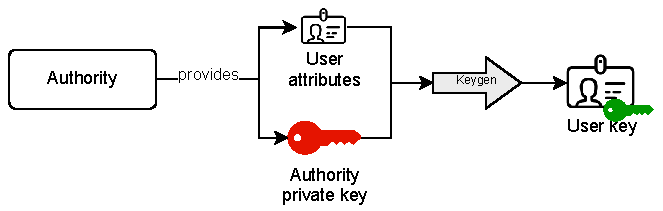
\includegraphics[width=\textwidth]{images/diagrams/keygen_diagram.pdf}
    \caption{Authorities issue keys to users based on their attributes.}
\end{figure}

\end{frame}
    \begin{frame}
    \frametitle{Encryption}
    \begin{figure}
        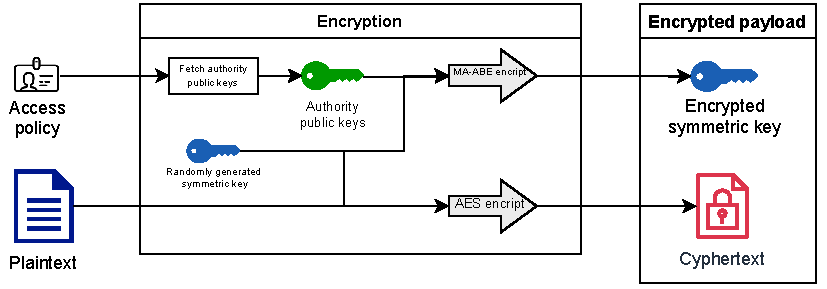
\includegraphics[width=\textwidth]{images/diagrams/encryption_diagram.pdf}
        \caption{The hybrid process combines MA-ABE for the symmetric key and AES for the payload.}
    \end{figure}
\end{frame}
        
\begin{frame}
    \frametitle{Decryption Process}
    \begin{itemize}
        \item To decrypt data, a user must possess a set of attribute keys that satisfies the access policy defined during encryption.
        \item The user first decrypts the symmetric key using their MA-ABE keys and then uses the symmetric key to decrypt the payload with AES.
    \end{itemize}
    \begin{figure}
        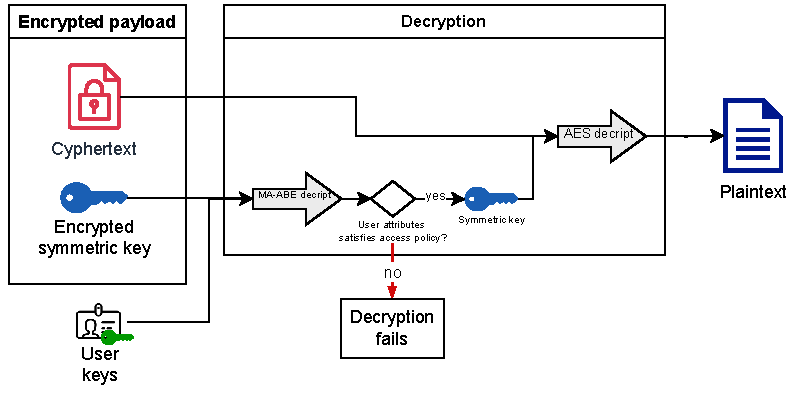
\includegraphics[width=0.8\textwidth]{images/diagrams/decryption_diagram.pdf}
        \caption{The decryption workflow enforces the access policy by requiring valid attribute keys to access the data.}
    \end{figure}
\end{frame}


% --- Experimental Setup ---
\section{Experimental Setup}

\begin{frame}
    \frametitle{Evaluation Strategy and Tools}
    The evaluation aimed to measure performance, scalability, and cryptographic overhead.
    \begin{itemize}
        \item A RESTful API was developed to provide endpoints for all cryptographic operations.
        \item \textbf{Locust} was used for load testing to simulate concurrent users.
        \item \textbf{Gunicorn} managed concurrent requests with configurable workers and threads.
        \item \textbf{Charm-Crypto} provided the implementation of the MaabeRW15 scheme for MA-ABE.
        \item \textbf{Flask}, \textbf{Flask-RESTX}, and \textbf{Redis} were used for the API and key management.
        \item All services were containerized with \textbf{Docker} for reproducibility.
    \end{itemize}
\end{frame}

% --- Results and Discussion ---
\section{Results and Discussion}

\begin{frame}
    \frametitle{Concurrency Analysis}
    \begin{itemize}
        \item The system scales effectively with the number of \textbf{processes (workers)} but does not benefit from multi-threading due to Python's Global Interpreter Lock (GIL).
        \item Optimal performance was achieved with 25 workers and 1 thread, which was used for subsequent tests.
    \end{itemize}
    \begin{figure}
        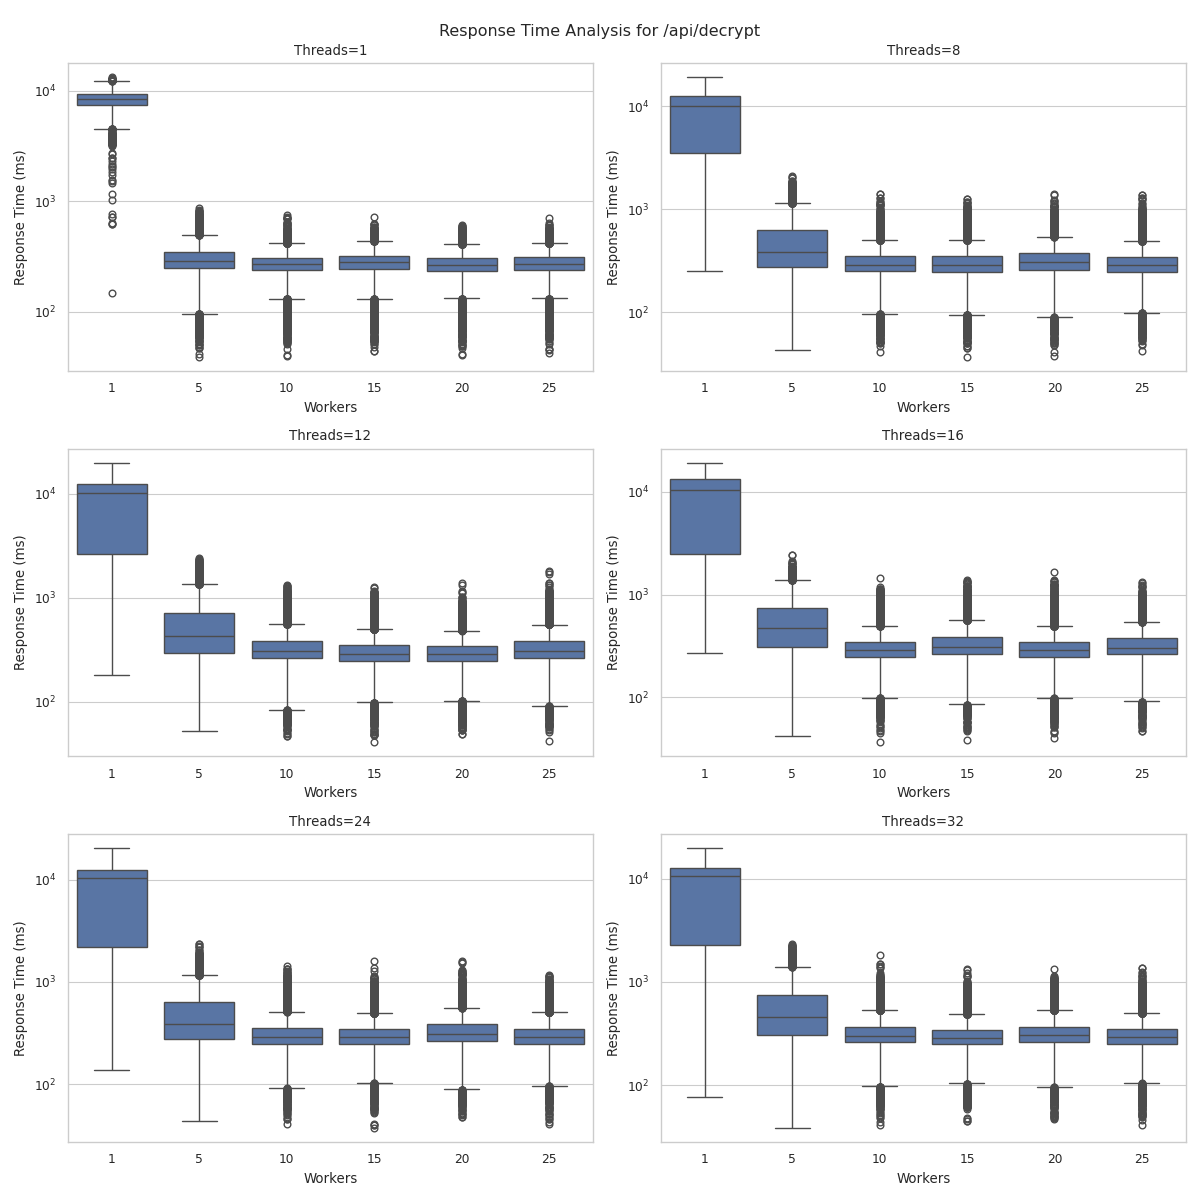
\includegraphics[width=0.8\textwidth]{images/phase1/api_decrypt/response_time_threads_summary.png}
        \caption{Decryption response time decreases as the number of workers increases (threads fixed at 1).}
    \end{figure}
\end{frame}

\begin{frame}
    \frametitle{Payload Size and Policy Complexity}
    \begin{itemize}
        \item \textbf{Payload Size:} Response times increase with larger payloads, but the hybrid approach remains efficient, confirming its suitability for large datasets.
        \item \textbf{Policy Complexity:} Response times, especially for decryption, increase with the number of attributes in the access policy, highlighting a trade-off between security granularity and performance.
    \end{itemize}
        \begin{figure}
        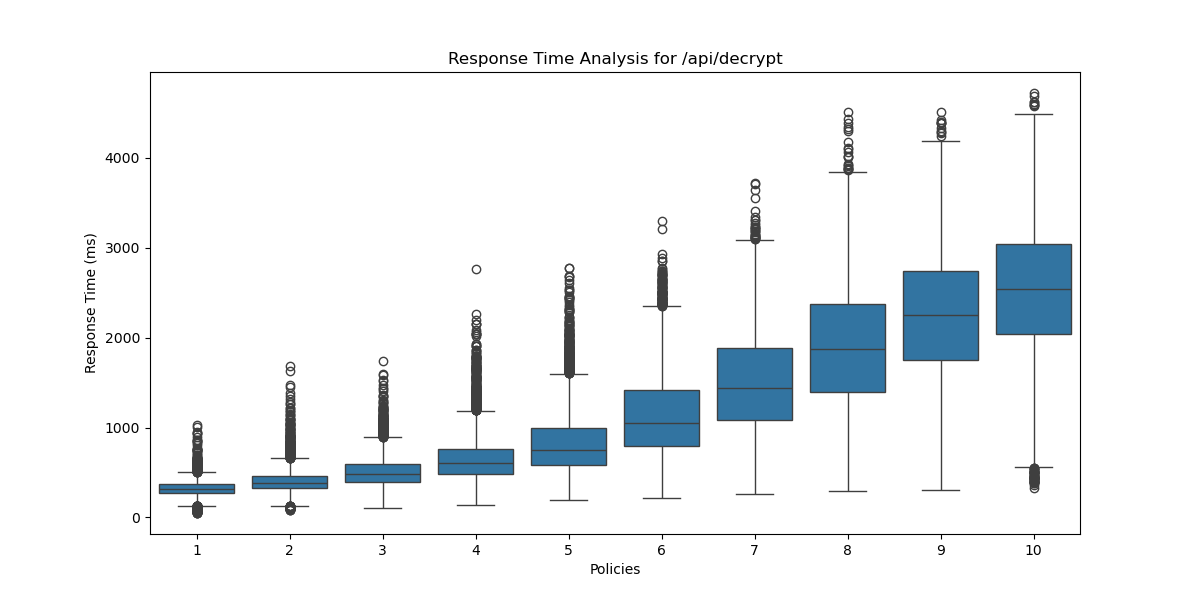
\includegraphics[width=\textwidth]{images/phase4/response_time_api_decrypt.png}
        \caption{Decryption response time for different policy sizes.}
    \end{figure}
\end{frame}

\begin{frame}
    \frametitle{User Load and Key Size}
    \begin{itemize}
        \item \textbf{User Load:} Performance degrades at high concurrency levels, showing the system handles moderate user loads well.
        \item \textbf{Key Size:} User key size grows linearly with the number of attributes, which has implications for storage and network bandwidth in a decentralized system like IPFS.
    \end{itemize}
    \begin{figure}
        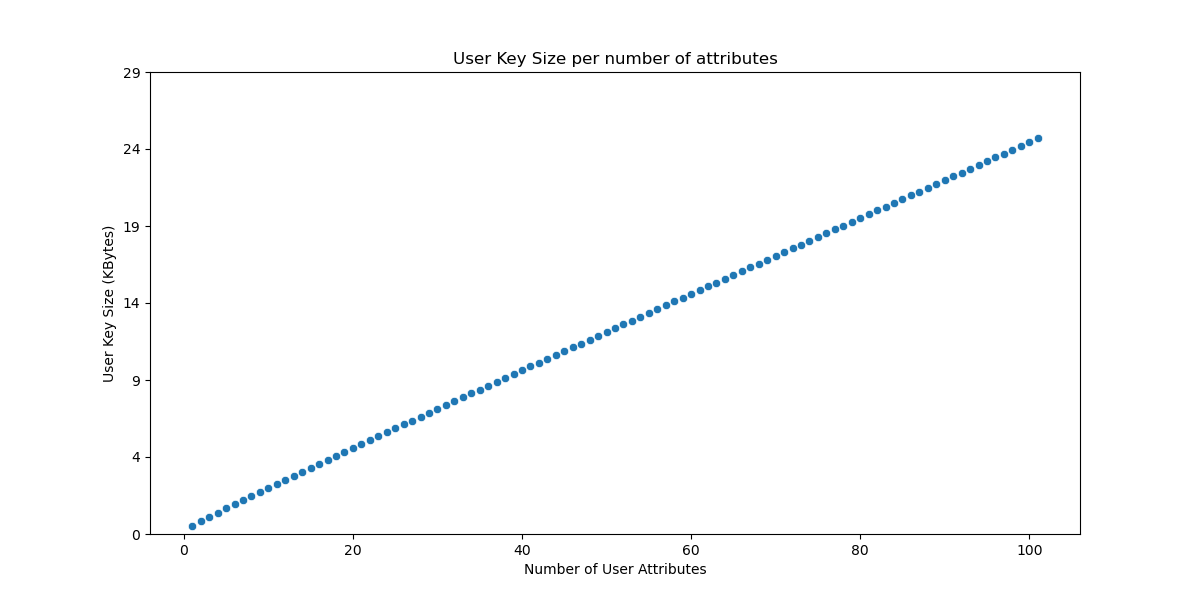
\includegraphics[width=0.9\textwidth]{images/key_size_analysis/user_key_size_analysis.png}
        \caption{User key size for different numbers of attributes.}
    \end{figure}
\end{frame}

% --- Conclusion ---
\section{Conclusion and Future Work}

\begin{frame}
    \frametitle{Conclusion}
    \begin{itemize}
        \item This thesis successfully addressed a critical gap in HIoT data security by proposing, implementing, and evaluating a hybrid MA-ABE and AES cryptographic scheme.
        \item The evaluation confirmed that the proposed solution is a viable and effective method for enforcing robust, fine-grained access control in decentralized HIoT systems.
        \item The results highlight a practical trade-off between security granularity and performance, providing valuable insights for real-world deployment.
    \end{itemize}
\end{frame}

\begin{frame}
    \frametitle{Future Work}
    \begin{itemize}
        \item Full integration with the decentralized storage framework by \citeonline{laura2023} and end-to-end evaluation in a distributed environment.
        \item Optimization for handling binary data (e.g., medical images) directly, to reduce encoding overhead and improve efficiency.
        \item Exploration of alternative key storage mechanisms to reduce I/O bottlenecks.
        \item Comparison with other MA-ABE schemes to further optimize performance.
    \end{itemize}
\end{frame}

\begin{frame}[allowframebreaks]
    \frametitle{References}
    \bibliography{biblio}
\end{frame}

% --- Thank you ---
\begin{frame}
    \frametitle{Obrigado!}
    \begin{center}
        \Large Questions?
    \end{center}
    \vspace{2cm}
    \InfContacts
\end{frame}


\end{document}